\documentclass[10pt,twocolumn,letterpaper]{article}

\usepackage{iccv}
\usepackage{times}
\usepackage{epsfig}
\usepackage{graphicx}
\usepackage{amsmath}
\usepackage{amssymb}
\usepackage{authblk}

\usepackage{mystyle}
% Include other packages here, before hyperref.

% If you comment hyperref and then uncomment it, you should delete
% egpaper.aux before re-running latex.  (Or just hit 'q' on the first latex
% run, let it finish, and you should be clear).
\usepackage[pagebackref=true,breaklinks=true,letterpaper=true,colorlinks,bookmarks=false]{hyperref}

\iccvfinalcopy % *** Uncomment this line for the final submission

\def\iccvPaperID{4160} % *** Enter the ICCV Paper ID here
\def\httilde{\mbox{\tt\raisebox{-.5ex}{\symbol{126}}}}

% Pages are numbered in submission mode, and unnumbered in camera-ready
% \ificcvfinal\pagestyle{empty}\fi
\begin{document}

%%%%%%%%% TITLE
\title{Deep Parametric Shape Predictions using Distance Fields}

\author{Dmitriy Smirnov$^1$, Matthew Fisher$^2$, Vladimir G. Kim$^2$, Richard Zhang$^2$, Justin Solomon$^1$\\
$^1$Massachusetts Institute of Technology, $^2$Adobe Research}

\maketitle
%\thispagestyle{empty}


%%%%%%%%% ABSTRACT
\begin{abstract}
Many tasks in graphics and vision demand machinery for converting shapes into representations with sparse sets of parameters; these representations facilitate rendering, editing, and storage. When the source data is noisy or ambiguous, however, artists and engineers often manually construct such representations, a tedious and potentially time-consuming process. While advances in deep learning have been successfully applied to noisy geometric data, the task of generating parametric shapes has so far been difficult for these methods. Hence, we propose a new framework for predicting parametric shape primitives using deep learning.  We use distance fields to transition between shape parameters like control points and input data on a raster grid. We demonstrate efficacy on 2D and 3D tasks, including font vectorization and surface abstraction.
\end{abstract}


\section{Introduction}

The creation, modification, and rendering of vector graphics and parametric shapes is a fundamental problem of interest to engineers, artists, animators, and designers. Such representations offer distinct advantages over other models. By expressing a shape as a collection of primitives, we are able to apply transformations easily, to identify correspondences, and to render at arbitrary resolution, all while having to store only a sparse representation.

It is often useful to generate a parametric model from data that does not directly correspond to the target geometry and contains imperfections or missing parts. This can be an artifact of noise, corruption, or human-generated input; often, an artist intends to create a precise geometric object but produces one that is ``sketchy'' and ambiguous. Hence, we turn to machine learning methods, which have shown success in inferring structure from noisy data.

Convolutional neural networks (CNNs) achieve state-of-the-art results in vision tasks such as image classification~\cite{krizhevsky2012imagenet}, segmentation~\cite{long2015fully}, and image-to-image translation~\cite{isola2017image}. CNNs, however, operate on \emph{raster} representations. Grid structure is fundamentally built into convolution as a mechanism for information to travel between layers of a deep network. This structure is leveraged during training to optimize performance on a GPU. Recent deep learning pipelines that output vector shape primitives \cite{tulsiani2017learning} have been significantly less successful than pipelines for analogous tasks on raster images or voxelized volumes. 

A challenge when applying deep learning to parametric geometry is the combination of Eulerian and Lagrangian representations.  CNNs process data in an \emph{Eulerian} fashion in that they apply fixed operations to a dense grid of values; Eulerian shape representations like indicator functions come as values on a fixed grid.  Parametric shapes, on the other hand, use sparse sets of parameters like control points to express geometry. In contrast to stationary Eulerian grid points, this \emph{Lagrangian} representation moves with the shape.  Navigating the transition from Eulerian to Lagrangian geometry is a key step in any learning pipeline for the problems above, a task we consider in detail.

We propose a deep learning framework for predicting parametric shapes, addressing the aforementioned issues. By analytically computing a distance field to the primitives at each training iteration, we formulate an Eulerian version of the Chamfer distance, a common metric for geometric similarity.  Our metric can be computed efficiently and does not require sampling points from the predicted or target shapes. Beyond accelerating evaluation of existing loss functions, our distance field enables alternative loss functions that are sensitive to specific geometric qualities like alignment.

We apply our new framework in the 2D context to a diverse dataset of fonts. We train a network that takes in a raster image of a glyph and outputs a representation as a collection of B\'ezier curves. This maps glyphs onto a common set of parameters that can be traversed intuitively. We use this embedding for font exploration and retrieval, correspondence, and unsupervised interpolation.

We also show that our approach works in 3D. With surface primitives in place of curves, we perform volumetric abstraction on ShapeNet \cite{shapenet2015}, inputting an image or a distance field and outputting parametric primitives that approximate the model. This output can be rendered at any resolution or converted to a mesh; it also can be used for segmentation.

\noindent\textbf{Contributions.} We present a technique for predicting parametric shapes from 2D and 3D raster data, including:
\begin{itemize}
    \item a \emph{general distance field loss function} allowing definition of several losses based on a common formulation;
    \item application to 2D \emph{font glyph vectorization}, with application to correspondence, exploration, retrieval, and repair;
    \item application to 3D \emph{surface abstraction}, with results for different primitives and constructive solid geometry (CSG) as well as application to segmentation.
\end{itemize}

\section{Related Work}

\paragraph*{Font exploration and manipulation.}
Designing or even finding a font can be tedious using generic vector graphics tools. Certain geometric features distinguish letters from one another across fonts, while others distinguish fonts from one another. Due to these difficulties and the presence of large font datasets, font exploration, design, and retrieval have emerged as challenging problems in graphics and learning.

Previous exploration methods categorize and organize fonts via crowdsourced attributes \cite{o2014exploratory} or embed fonts on a manifold using purely geometric features \cite{campbell2014learning,Balashova18}. Instead, we leverage deep vectorization to automatically generate a sparse representation for each glyph. This enables exploration on the basis of general shape rather than fine detail.

Automatic font generation methods usually fall into two categories. Rule-based methods \cite{suveeranont2010example,phan2015flexyfont} use engineered decomposition and reassembly of glyphs into parts. Deep learning approaches \cite{azadi2018multi,upchurch2016z} produce raster images, with limited resolution and potential for image-based artifacts, making them unfit for use as glyphs. We apply our method to edit existing fonts while retaining vector structure and demonstrate vectorization of glyphs from partial and noisy data, \ie, raster images from a generative model.

\paragraph*{Parametric shape collections.} As the number of publicly-available 3D models grows, methods for organizing, classifying, and exploring models become crucial. Many approaches decompose models into modular parametric components, commonly relying on prespecified templates or labeled collections of specific parts \cite{kim2013learning,shen2012structure,ovsjanikov2011exploration}. Such shape collections prove useful in domain-specific applications in design and manufacturing \cite{schulz2017retrieval,umetani2012guided}.  Our deep learning pipeline allows generation of parametric shapes to perform these tasks. It works quickly on new inputs at test time and is generic, handling a variety of modalities without supervision and producing different output types.

\paragraph*{Deep 3D reconstruction.} Combining multiple viewpoints to reconstruct 3D geometry is crucial in applications like robotics and autonomous driving  \cite{fuentes2015visual,seitz2006comparison,su2015multi}. Even more challenging is inference of 3D structure from one input. Recent deep networks can produce point clouds or voxel occupancy grids given a single image \cite{fan2017point,choy20163d}, but their output suffers from fixed resolution.

Learning signed distance fields defined on a voxel grid \cite{dai2017shape,stutz2018learning} or directly \cite{park2019deepsdf} allows high-resolution rendering but requires surface extraction; this representation is neither sparse nor modular. Liao \etal address the rendering issue by incorporating marching cubes into a differentiable pipeline, but the lack of sparsity remains problematic, and predicted shapes are still on a voxel grid \cite{liao2018deep}

Parametric 3D shapes offer a sparse, non-voxelized solution. Methods for converting point clouds to geometric primitives achieve high-quality results but require supervision, either relying on existing data labelled with primitives \cite{li2018supervised, niu2018im2struct} or prescribed templates \cite{ganapathi2018parsing}. Tulsiani \etal output cuboids but are limited in output type \cite{tulsiani2017learning}. Groueix \etal output primitives at any resolution, but their primitives are not naturally parameterized or sparsely represented \cite{groueix2018atlasnet}.

\section{Preliminaries}
\label{sec-prelim}

Let $A, B \subset \R^n$ be two smooth (measurable) shapes. Let $X$ and $Y$ be two point sets sampled uniformly from $A$ and $B$. The \emph{directed Chamfer distance} between $X$ and $Y$ is
\begin{equation}\label{eq:chamferdir}
    \Ch_\mathrm{dir}(X,Y) = \sum_{x \in X} \min_{y \in Y} \dd(x,y),
\end{equation}
and the \emph{symmetric Chamfer distance} is defined as
\begin{equation}\label{eq:chamfer}
    \Ch(X,Y) = \Ch_\mathrm{dir}(X,Y) + \Ch_\mathrm{dir}(Y,X).
\end{equation}
\noindent It was proposed for computational applications in \cite{borgefors1984distance} and has been used as a loss function assessing similarity of a learned shape to ground truth in deep learning \cite{tulsiani2017learning, fan2017point, liu2004hand, groueix2018atlasnet}.

We also define \emph{variational directed Chamfer distance}
\begin{equation}
    \Ch_\mathrm{dir}^\mathrm{var}(A,B) = \int_A \inf_{y \in B} \|x-y\|_2\,\dint x,
\end{equation}
with \emph{variational symmetric Chamfer distance} $\Ch(A,B)^\mathrm{var}$ defined analogously,   extending \eqref{eq:chamferdir} and \eqref{eq:chamfer} to smooth objects. We use this to relate our proposed loss to Chamfer distance.

\begin{figure}[t!]
    \centering
    \begin{subfigure}[b]{0.6\linewidth}
        \includegraphics[width=\linewidth]{figures/chamfer2}
        \caption{Sampling}
        \label{fig:chamfer-sampling}
        \centering
    \end{subfigure}
    \begin{subfigure}[b]{0.35\linewidth}
        \includegraphics[width=\linewidth]{figures/chamfer1}
        \caption{Alignment}
        \label{fig:chamfer-normals}
    \end{subfigure}
    \caption{Drawbacks of Chamfer distance. In (a), sampling from B\`ezier curve $B$ (blue) by uniformly sampling in parameter space yields disproportionately many points at the high-curvature area, resulting in a low Chamfer distance to the segments of $A$ (orange) despite geometric dissimilarity. In (b), two sets of nearly-orthogonal line segments have near-zero Chamfer distance despite misaligned normals.\vspace{-0.1in}}
\end{figure}

If points are sampled uniformly, under relatively weak assumptions about $A$ and $B$, $\Ch(X,Y) \to 0$ iff $A = B$, as the sizes of the sampled point sets grow. Thus, it is a reasonable shape matching metric.
Chamfer distance, however, has fundamental drawbacks:
\begin{itemize}[leftmargin=*]
    \item It is highly dependent on the sampled points and sensitive to non-uniform sampling, as in Figure~\ref{fig:chamfer-sampling}.
    \item It is slow to compute. For each $x$ sampled from $A$, it is necessary to find the closest $y$ sampled from $B$, a quadratic-time operation when implemented na\"ively. Efficient structures like $k$-d trees are not well-suited to GPUs.
    \item It is agnostic to normal alignment. As in Figure~\ref{fig:chamfer-normals}, the Chamfer distance between a dense set of vertical lines and a dense set of horizontal lines approaches zero.
\end{itemize}
Our method does not suffer from these disadvantages.

\section{Method}
\label{sec-method}

Beyond architectures for particular tasks, we introduce a framework for formulating loss functions suitable for learning placement of parametric shapes in 2D and 3D; our formulation not only encapsulates Chamfer distance---and suggests a means of accelerating its computation---but also leads to stronger loss functions that improve performance on a variety of tasks. We start by defining a general loss on distance fields and propose three specific losses.

\subsection{General Distance Field Loss}

Given $A,B\subseteq\R^n$, let $\dd_A, \dd_B : \R^n \to \R_+$ measure distance from each point in $\R^n$ to $A$ or $B$, respectively, $\dd_A(x)\eqdef \inf_{y\in A} \|x-y\|_2$. In our experiments, $n \in \{2,3\}.$
Let $S \subseteq \R^n$ be a bounded set with $A,B \subseteq S$. We define the \emph{general distance field loss} as
\begin{equation}
\label{gdf-loss}
    \LL_\Psi[A, B] = \int_{x\in S} \Psi_{A,B}(x)\,\dint V(x),
\end{equation}
for some measure of discrepancy $\Psi$. Note that we represent $A$ and $B$ only by their respective distance functions, and the loss is computed over $S$.

Let $\Phi \in \R^p$ be a collection of parameters defining a shape. For instance, a parametric shape may consist of B\'ezier curves, in which case $\Phi$ contains a list of control points. Let $\dd_\Phi : \R^n \to \R_+$ be the distance to the shape defined by $\Phi$. Given a target object $T$ with distance function $\dd_T$, we formulate fitting a parametric shape to approximate  $T$ w.r.t.\ $\Psi$ as minimizing
\begin{equation}\label{eq:generalloss}
    f_\Psi(\Phi) = \LL_\Psi[\Phi, T].
\end{equation}
For optimal shape parameters, $\hat\Phi := \argmin_\Phi f_\Psi(\Phi)$.  We propose three discrepancy measures, providing loss functions that capture different geometric features.

\subsection{Surface Loss}

We define surface discrepancy to be
\begin{equation}
\Psi^\textrm{surf}_{A,B}(x)\!=\!\delta\{\ker \dd_A\}(x)\!\dd_B(x)\!+\!\delta\{\ker \dd_B\}(x)\!\dd_A(x)
\end{equation}
where $\delta\{X\}$ is the Dirac delta defined uniformly on $X$, and $\ker f$ denotes the zero level-set of $f$. 
%
$\Psi^\textrm{surf}$ is only nonzero where the shapes do not match, making it sensitive to fine details in the matching:

\begin{prop}
The symmetric variational Chamfer distance between $A,B \subset \R^n$ equals the corresponding surface loss between, \ie, $\Ch^\mathrm{var}(A,B) = \LL_{\Psi^\textrm{surf}_{A,B}}$.
\end{prop}

\noindent Unlike the Chamfer distance, the discrete version of our surface loss can be approximated efficiently on GPU without sampling points from either the parametric or target shape.

\subsection{Global Loss}

We define global discrepancy to be
\begin{equation}
   \Psi^\textrm{glob}_{A,B}(x) = |\dd_A(x) - \dd_B(x)|^2.
\end{equation}
Minimizing $\LL_{\Psi^\textrm{glob}_{A,B}}$ is equivalent to minimizing the $L_2$ distance between $\dd_A$ and $\dd_B$. $f_{\Psi^\textrm{glob}}(\Phi)$ increases quadratically in distance between the shape defined by $\Phi$ and the target shape. Thus, minimizing $f_{\Psi^\textrm{glob}}$ encourages global alignment, quickly placing the parametric primitives close to the target and accelerating convergence.

\subsection{Normal Alignment Loss}

We define normal alignment discrepancy to be
\begin{equation}
    \Psi^\textrm{align}_{A,B}(x) = \|\nabla \dd^2_A(x) - \nabla \dd^2_B(x)\|^2_2.
\end{equation}
Minimizing $f_{\Psi^\textrm{align}}$ aligns normals of the predicted primitives to those of the target. Following Figure~\ref{fig:chamfer-normals}, if $A$ contains dense vertical lines and $B$ contains horizontal lines, $\LL_{\Psi^\textrm{align}_{A,B}}$ is large while $\Ch(A,B) \approx 0$.


\subsection{Final Loss Function}

\begin{figure}[t]
\centering
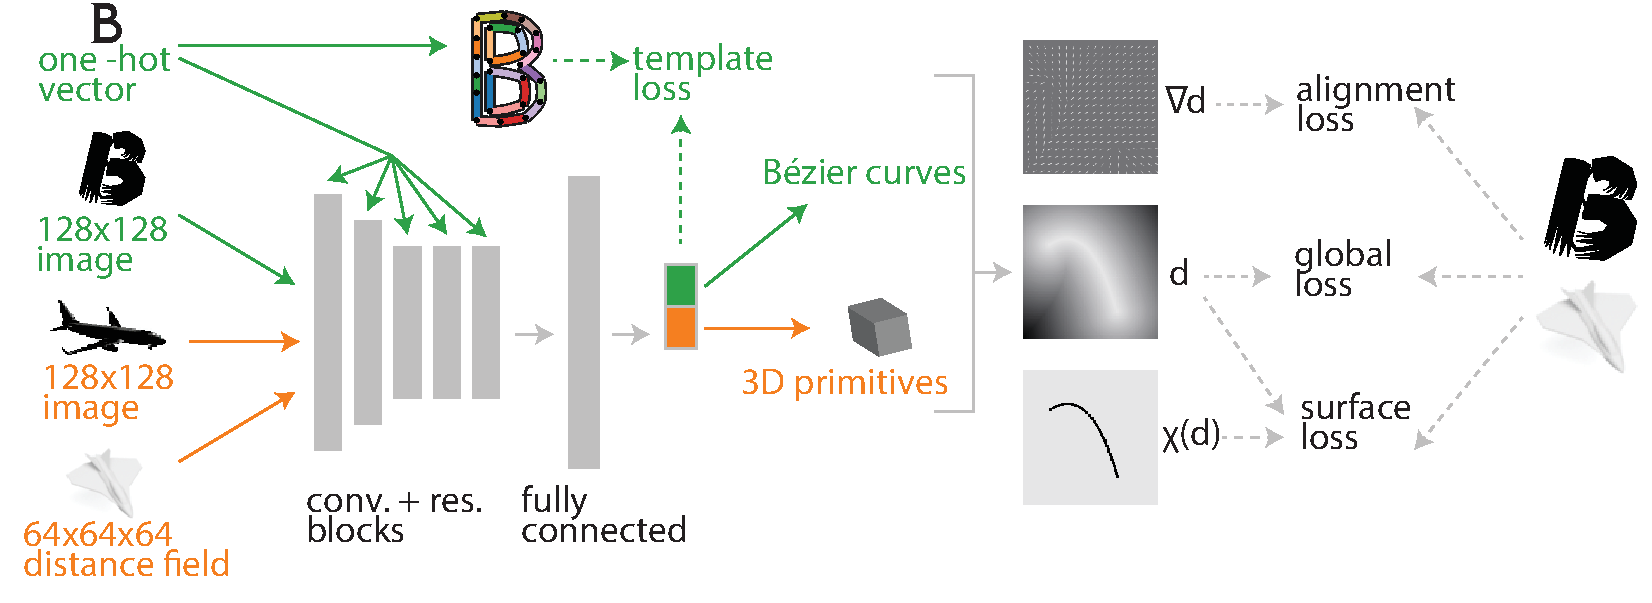
\includegraphics[width=\linewidth]{figures/architecture}\vspace{-0.1in}
\caption{An overview of our pipelines---font vectorization (green) and volumetric primitive prediction (orange).\vspace{-0.1in}}
\label{fig:architecture}
\end{figure}

The general distance field loss and the specific discrepancy measures proposed thus far are differentiable w.r.t\ the shape parameters $\Phi$, as long as the distance function $\dd_
\Phi$ is differentible w.r.t.\ $\Phi$. Thus, they are well-suited to be optimized by a deep network that predicts parametric shapes. To discretize, we simply redefine~\eqref{gdf-loss} to be
\begin{equation}
	\LL_\Psi[A, B] = \sum_{x \in G} \Psi_{A,B}(x),
\end{equation}
where $G$ is a 2D or 3D grid. Thus, we minimize a weighted sum of $f_\Psi(\Phi)$ across the $\Psi$ defined in \S\ref{sec-method}:
\begin{equation}
\Psi = \Psi^\text{glob}+\alpha^\textrm{surf}\Psi^\text{surf}+\alpha^\textrm{align}\Psi^\text{align}.
\end{equation}
We use $\alpha^\textrm{surf}=1$ and $\alpha^\textrm{align}=0.001$ across experiments. In 3D experiments, we decay the global loss term exponentially by a factor 0.5 every 500 iterations.

\subsection{Network architecture}
The network takes a $128\!\times\!128$ image or a $64\!\times\!64\!\times\!64$ distance field as input and outputs a parametric shape. We use the same architecture for 2D and 3D, following advances in network architecture design. Let \texttt{c5s2-64} be a convolutional layer with 64 filters of $5\!\times\!5$ evaluated at stride $2$, \texttt{Rx7} be 7 residual blocks~\cite{he2016identity,he2016deep} of size $3\!\times\!3$ (keeping filter count constant), and \texttt{fc-512} be a fully-connected layer. To increase receptive field without dramatically increasing parameter count, we also use dilated convolution \cite{yu2015multi, chen2018deeplab} in residual blocks. We use \texttt{ELU}~\cite{clevert2015fast} after all linear layers except the last. We use \texttt{LayerNorm}~\cite{ba2016layer} after each conv and residual layer, except the first. Our encoder architecture is: {\small
\texttt{c5s1-32,} %1 - 32
\texttt{c3s2-64,} %2 - 64
\texttt{c3s1-64,} %3 - 64
\texttt{c3s2-128,} %4 - 128
\texttt{c3s1-128,} %5 - 128
\texttt{c3s1-128,}
\texttt{c3s2-256,} %6 - 256
\texttt{Rx7,} %7
\texttt{c3s2-256,} %8 - 256
\texttt{Rx1,} % 9
\texttt{c3s2-256,} %10 - 256
\texttt{Rx1,} % 11
\texttt{fc-512, fc-N}}, where \texttt{N} is the dimension of our target parameterization. Our pipeline is illustrated in Figure~\ref{fig:architecture}. We train each network on a single Tesla K80 GPU, using Adam \cite{kingma2014adam} with learning rate $10^{-4}$ and batch size 16.

\begin{figure*}[t!]
    \centering
    \begin{subfigure}[b]{.45\linewidth}
        \centering
        
\includegraphics[width=\linewidth]{figures/abc_plain.pdf}
        \caption{Plain font glyphs}
        \label{fig:abc-plain}
    \end{subfigure}
    \hspace{8mm}
    \begin{subfigure}[b]{.45\linewidth}
        
\includegraphics[width=\linewidth]{figures/abc_decorative}
        \caption{Decorative font glyphs}
        \label{fig:abc-decorative}
    \end{subfigure}\vspace{-.12in}
    \caption{Vectorization of various glyphs. For each we show the raster input (top left, gray) along with the vectorization (colored curves) superimposed. When the input has simple structure (a), we recover an accurate vectorization. For fonts with decorative details (b), our method places template curves to capture overall structure. Results are taken from the test dataset.\vspace{-.18in}}
\end{figure*}


\section{2D: Font Exploration and Manipulation}

We demonstrate our method in 2D for font glyph vectorization. Given a raster image of a glyph, our network outputs control points that form a collection of quadratic B\'ezier curves approximating its outline. When used on a glyph of a simple font (non-decorative, \eg, sans-serif), our method recovers nearly the exact original vector representation. From a decorative glyph with fine-grained detail, however, we recover a good approximation of the glyph's shape using relatively few B\'ezier primitives and a consistent structure. This process can be interpreted as projection onto a common sparse latent space of control points.

We first describe our choice of primitives as well as the computation of their distance fields. We introduce a template-based approach to allow our network to better handle multimodal data (different letters) and test several applications.

\subsection{Approach}

\subsubsection{Primitives}

We wish to use a 2D parametric shape primitive that is sparse and expressive and admits an analytic distance field. Our choice satisfying these requirements is the \emph{quadratic B\`ezier curve}, which we will refer to as \emph{curve}, parameterized by control points $a, b, c \in \R^2$ and defined by $B(t) = (1-t)^2a + 2(1-t)tb + t^2c,$ for $0 \le t \le 1$. We represent 2D shapes as the union of $n$ curves parameterized by $\Phi = \{a_1, b_1, c_1, \ldots, a_n, b_n, c_n\}$, where $a_i, c_i, b_i \in \R^2$.

\begin{prop}
Given a curve $B$ parameterized by $a,b,c \in \R^2$ and a point $p \in \R^2$, the $\hat t \in \R$ such that $B(\hat t)$ is the closest point on the curve to $p$ satisfies the following:
\begin{equation}
\label{curve-dist}
\begin{split}
\langle B, B \rangle \hat t^3 + 3 \langle A, B \rangle \hat t^2 &+ (2\langle A, A \rangle + \langle B, a - p \rangle)\hat t \\&+ \langle A, a - p \rangle = 0,
\end{split}
\end{equation}
where $A = b-a$ and $B = c - 2b + a$.
\end{prop}

Thus, evaluating the distance to a single curve $\dd(p, B_i) = \|p - B_i(\hat t)\|_2$ requires finding the roots of a cubic \cite{qin2006real}, which we can do analytically in constant time. To compute distance to the union of the curves, we take a minimum:
\begin{equation}
\dd_\Phi(p) = \min_{i=1}^n \dd_{B_i}(p).
\end{equation}

In addition to the control points, we predict a stroke thickness parameter for each curve. We use this parameter when computing the loss by ``lifting'' the predicted distance field and, consequently, thickening the curve---if a curve $B$ has stroke thickness $s$, we set $d^s_B(p) = \min(d_B(p)-s,0)$. While we do not visualize stroke thickness in our experiments, this approach allows the network to thicken curves to better match fine-grained decorative details (Figure~\ref{fig:abc-stroke}). This thickening is a simple and natural operation in our distance field representation; note that sampling-based methods do not provide a natural way to ``thicken'' the surfaces.

\begin{figure}[t]
\centering
\includegraphics[width=\linewidth]{figures/abc_stroke}\vspace{-.1in}
\caption{Glyphs with corresponding predicted curves rendered with predicted stroke thickness. The network thickens curves of to account for  stylistic details.\vspace{-0.1in}}
\label{fig:abc-stroke}
\end{figure}

\subsubsection{Templates}

Our training procedure is unsupervised, as we do not have ground truth curve annotations. To better handle the multimodal nature of our data without a separate network for each letter, we label each training example with its letter, passed as additional input to our network. This allows us to condition based on input class by concatenating a 26-dimensional one-hot vector to the input of each convolutional layer (after replicating to the appropriate spatial dimensions), a common technique for conditioning \cite{zhu2017toward}.

We choose a ``standard'' B\`ezier curve representation for each letter, which captures that letter's distinctive geometric and topological features, by designing 26 templates from a shared set of control points output by our network. A \emph{template} of class $\ell \in \{\textrm{A}, \ldots, \textrm{Z}\}$ is a collection of points $T_\ell = \{p_1, \ldots, p_n\} \subseteq \R^{2n}$ with corresponding \emph{connectivity} determining how points in $T_\ell$ are used to define curves. Since we predict glyph boundaries, our final curves form closed loops, allowing us to reuse endpoints.

\begin{figure}[t]
\centering
\begin{subfigure}[b]{0.47\linewidth}
\includegraphics[width=\linewidth]{figures/abc_templates}
\caption{Letter templates}
\label{fig:templates-abc}
\end{subfigure}
\begin{subfigure}[b]{0.47\linewidth}
    \centering
    \includegraphics[width=0.5\linewidth]{figures/simple_templates}
    \caption{Simple templates}
    \label{fig:simple_templates}
\end{subfigure}
\caption{Font glyph templates. These determine the connectivity and initialize the placement of the predicted curves.\vspace{-0.1in}}
\label{fig:templates}
\end{figure}

For extracting glyph boundaries from uppercase English letters, there are three connectivity types---one loop (\eg, \emph{C}), two loops (\eg, \emph{A}), and three loops (\emph{B}). We design templates such that the first loop has 15 curves and the other loops have 4 curves each. Our templates are shown in Figure~\ref{fig:templates}. We will show that while letter templates (a) are better able to specialize to the boundaries of each glyph, we still achieve good results for most letters with the simple templates (b), which also allow for establishing cross-glyph correspondences.

We use predefined templates together with our labeling of each training example for two purposes. First, connectivity is used to compute curve control points from the network output. Second, they provide a \emph{template loss}
\begin{equation}
\LL^\textrm{template}(c, x) = \alpha^\textrm{template}\gamma^{(t/s)} \| T_c -  h^t(x)\|_2^2,
\end{equation}
where $s \in \Z_+$,  $\gamma \in (0,1)$, and $t$ is the current iteration. This serves to initialize the network output, such that a training example of class $\ell$ initially maps to template letter $\ell$; as the loss decays during training, it acts as a regularizer. We choose $\alpha^\textrm{template}=1$, $\gamma=0.7$, and $s=300$. 

\subsection{Experiments}

We train our network on the 26 uppercase English letters extracted from nearly 10,000 fonts. The input is a raster image of a letter, and the target distance field to the boundary of the original vector representation is precomputed.

\subsubsection{Vectorization}

For any font glyph, our method generates a sparse vector representation, which robustly and accurately describes the glyph's structure while ignoring decorative and noisy details. For simple fonts comprised of few strokes, our representation is a nearly perfect vectorization, as in Figure~\ref{fig:abc-plain}.

For glyphs from decorative fonts, our method produces a meaningful representation. In such cases, a true vectorization would contain many curves with a large number of connected components. Our network places the sparse curve template to best capture the glyph's structure, as in Figure~\ref{fig:abc-decorative}.

Our method preserves semantic correspondences in our templates. The same curve is consistently used for the boundary of, \eg, the top of an \emph{I}. These correspondences persist \emph{across} letters for both letter templates and simple templates---see for example the \emph{E} and \emph{F} glyphs in Figure~\ref{fig:abc-plain} and \ref{fig:abc-decorative} and ``simple templates'' in Figure~\ref{fig:abc-ablation}.

We demonstrate robustness in Figure~\ref{fig:abc-loss} by quantizing our loss values and visualizing the number of examples for each value. Outliers corresponding to higher losses are generally caused by noisy data---they are either not uppercase English letters or have fundamentally uncommon structure.


\begin{figure}[t]
    \centering
    
\includegraphics[width=\linewidth]{figures/abc_nn2}
    
\includegraphics[width=\linewidth]{figures/abc_nn5}
    \caption{Nearest neighbors for a glyph in curve space, sorted by proximity. The query glyph is in orange.\vspace{-0.1in}}
    \label{fig:abc-nn}
\end{figure}

\subsubsection{Retrieval and Exploration}

Our sparse representation can be used to explore the space of glyphs, useful for artists and designers. By treating the control points as a metric space, we can perform nearest-neighbor lookups to retrieve fonts using Euclidean distance.

In Figure~\ref{fig:abc-nn}, for each query, we compute its curve representation and retrieve seven nearest neighbors in curve space. Because our representation uses geometric structure, we find fonts that are similar structurally, despite decorative and stylistic differences.

We can also consider a path in curve space starting at the curves for one glyph and ending at those for another. By sampling nearest neighbors along this trajectory, we interpolate between glyphs. As in Figure~\ref{fig:abc-interpolation}, this produces meaningful collections of fonts for the same letter and reasonable results when the start and end glyphs are different letters. Additional results are available in the supplementary material.

\begin{figure}[t]
    \centering
    
\includegraphics[width=\linewidth]{figures/abc_interpolation3}
    
\includegraphics[width=\linewidth]{figures/abc_interpolation4}
    \caption{Interpolating between fonts in curve space. The start and end are shown in orange and blue, resp., and nearest-neighbor glyphs to linear interpolants are shown in order.\vspace{-0.1in}}
    \label{fig:abc-interpolation} 
\end{figure}

\begin{figure}[t]
    \centering
    \includegraphics[width=0.7\linewidth]{figures/abc_loss}
    \caption{Number of examples per quantized loss value. We visualize the input and predicted curves for several outliers.\vspace{-0.1in}}
    \label{fig:abc-loss}
\end{figure}


Nearest-neighbor lookups in curve space also can help find a font matching desired geometric characteristics. A possible workflow is in Figure~\ref{fig:abc-exploration}---through incremental refinements of the curves the user can quickly find a font.

\begin{figure}[t]
    \centering
    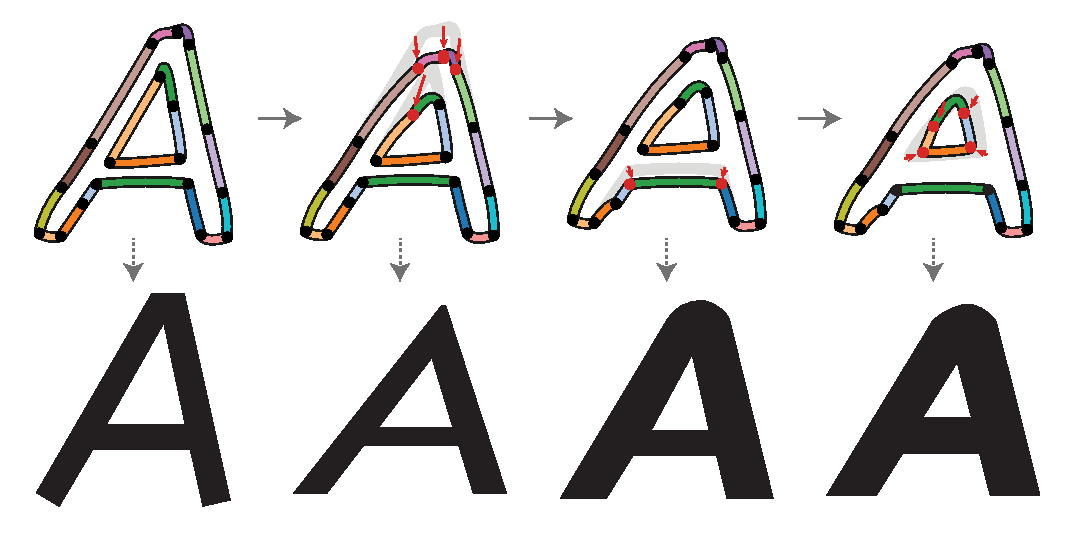
\includegraphics[width=0.6\linewidth]{figures/abc_exploration1}\vspace{-.1in}
    \caption{User-guided font exploration. At each edit, the nearest-neighbor glyph is displayed on the bottom. This lets the user explore the dataset through geometric refinements.\vspace{-0.1in}}
    \label{fig:abc-exploration}
\end{figure}


\subsubsection{Style and Structure Mixing}

Our sparse curve representation describes geometric structure, ignoring stylistic elements (\eg, texture, decorative details). We leverage this to warp a glyph with desired style to have a target structure of another glyph (Figure~\ref{fig:abc-analogies}).

\begin{figure}[t]
    \centering
    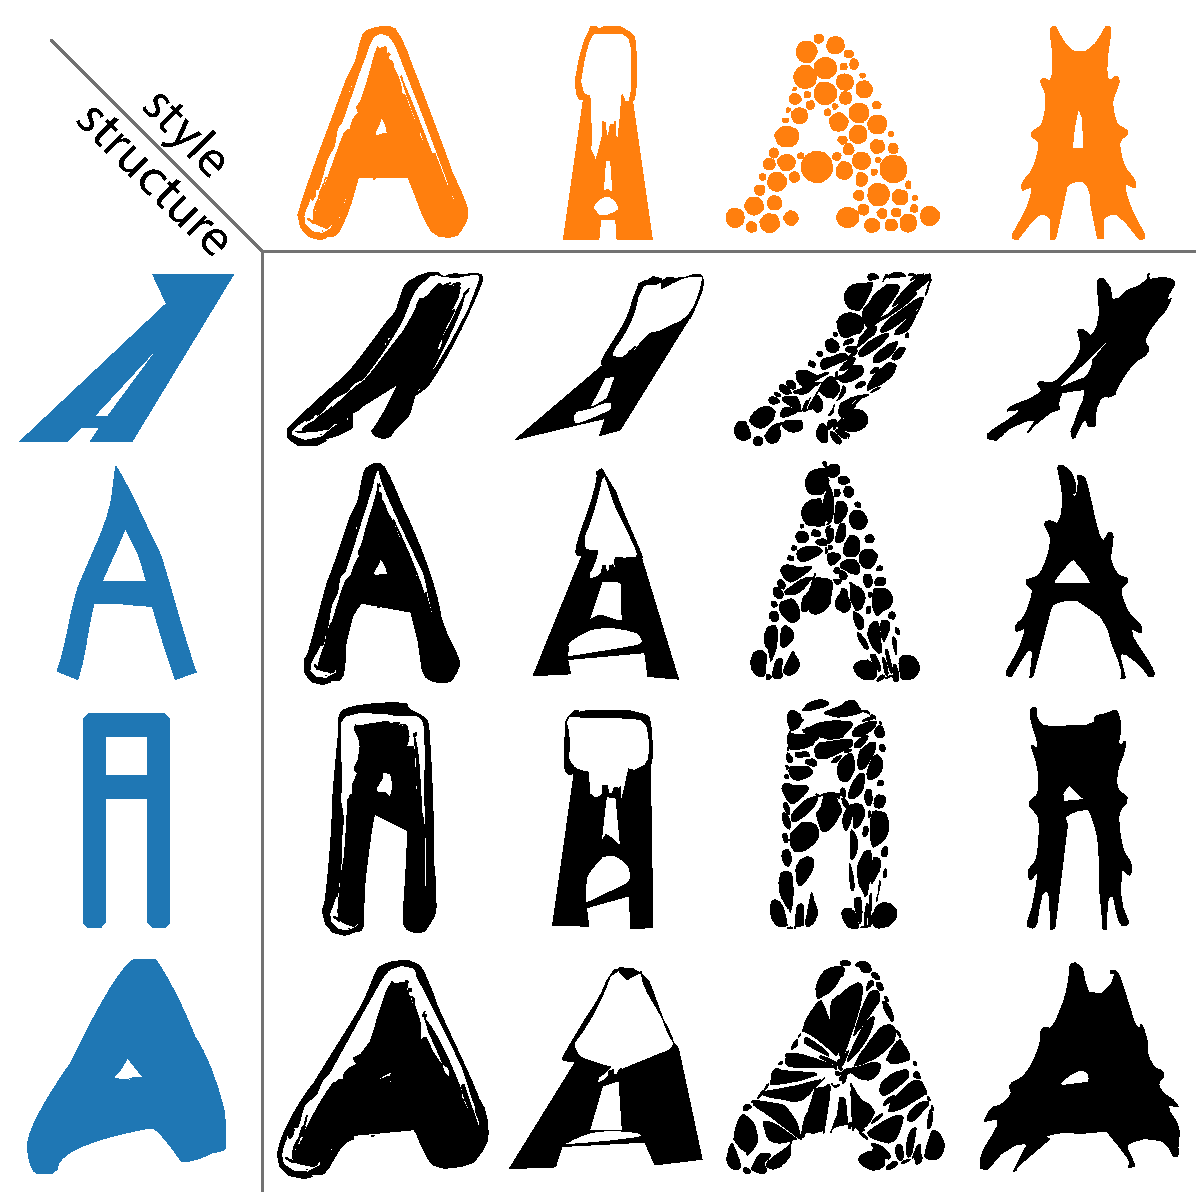
\includegraphics[width=0.7\linewidth]{figures/abc_analogies}\vspace{-.1in}
    \caption{Mixing of style (columns) and structure (rows) of the \emph{A} glyph from different fonts. We deform each starting glyph (orange) into the structure of each target glyph (blue).\vspace{-0.1in}}
    \label{fig:abc-analogies}
\end{figure}

We first generate the sparse curve representation for source and target glyphs. Since our representation uses the same set of curves, we can estimate dense correspondences and use them to warp original vectors of source glyph to conform to the shape of the target. For each point $p$ on the source, we find the closest point $q$ on the its sparse curve representation. We then compute the translation from  $q$ to the corresponding point on the target glyph's sparse representation and apply this translation to $p$.


\subsubsection{Repair}

Our system introduces a strong prior on glyph shape, allowing us to robustly handle noisy input. In \cite{azadi2018multi}, a generative adversarial network (GAN) generates new glyphs based on samples. The outputs, however, are raster images, often with noise and missing parts. Figure~\ref{fig:abc-gan} shows how our method can simultaneously vectorize and repair GAN-generated glyphs. Compared to a vectorization tool like Adobe Illustrator Live Trace, we infer missing data to reasonably fit the template. This post-processing step makes the glyphs from generative models usable starting points for font design.

\begin{figure}[t]
    \centering
    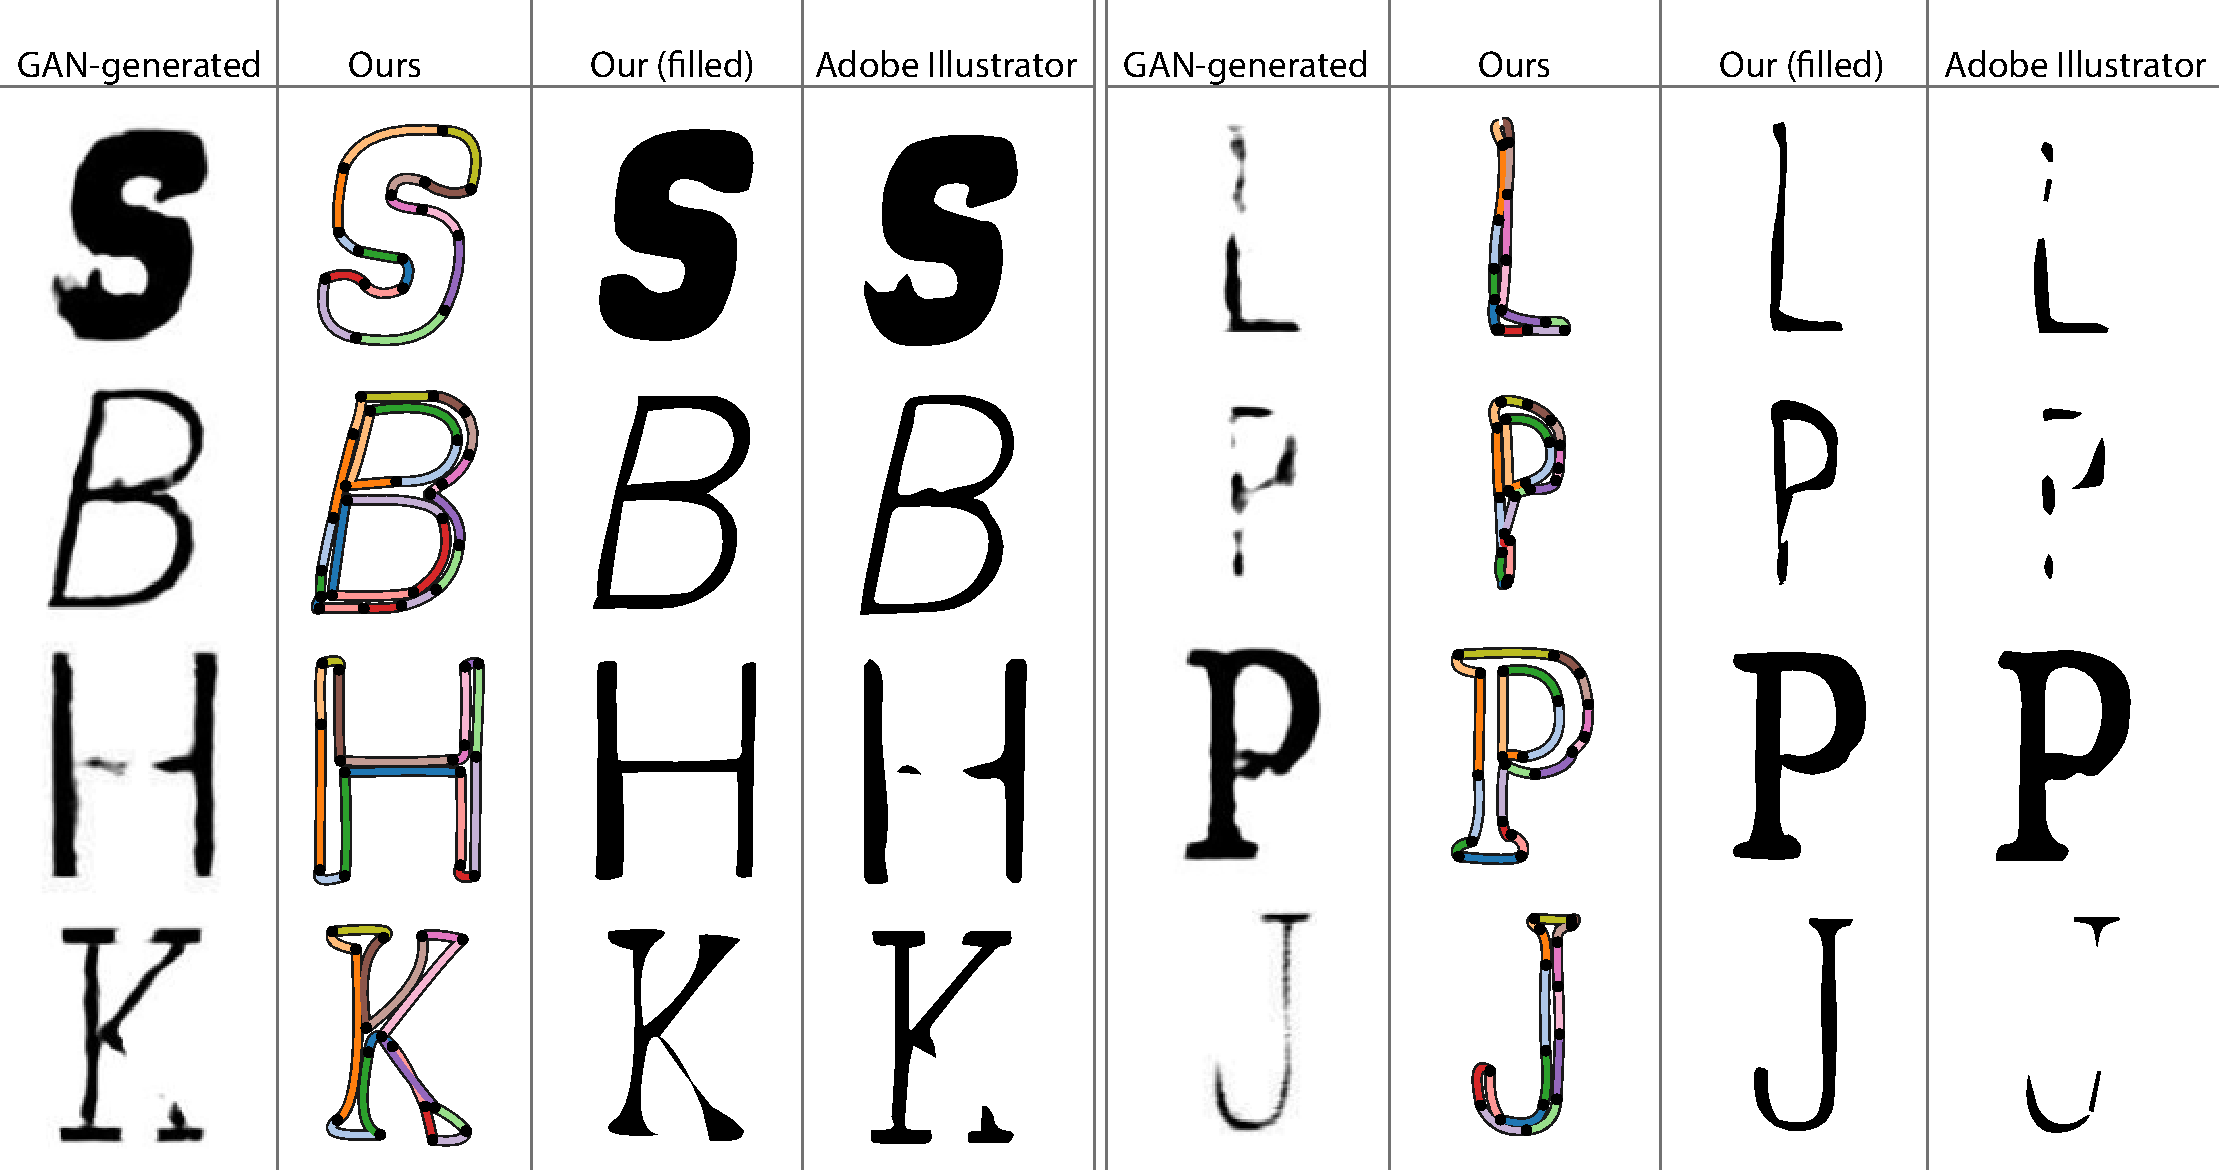
\includegraphics[width=\linewidth]{figures/abc_gan1}\vspace{-.1in}
    \caption{Vectorization of GAN-generated fonts from \cite{azadi2018multi}.\vspace{-0.1in}}
    \label{fig:abc-gan}
\end{figure}

\subsubsection{Comparison and Ablation Study}

We show a series of experiments that demonstrate the advantages of our loss over standard Chamfer distance as well as the contributions of each term in our loss. We demonstrate that while having 26 unique templates helps achieve better results, it is not crucial---we evaluate a network trained with  three ``simple templates" (Figure~\ref{fig:simple_templates}), which capture the three topology classes of our data.

\begin{table}[t]
    \centering
    \begin{tabular}{|c|c|c|}
         \hline
         Loss type & Sec/it & Average error \\
         \hline\hline
         Full model (ours) & 1.119 & 0.748 \\
         No global term (ours) & 1.111 & 0.817 \\
         No surface term (ours) & 1.109 & 0.761 \\
         No alignment term (ours) & 1.118 & 0.786 \\
         Simple templates (ours) & 1.127 & 0.789\\
         Chamfer & 1.950 & 0.910 \\
         \hline
    \end{tabular}
    \caption{Comparison between subsets of our full loss as well as standard Chamfer distance. Average error is Chamfer distance (in pixels on a $128\!\times\!128$ image) between predicted curves and ground truth, with points sampled uniformly. This demonstrates advantages of our loss over Chamfer distance and shows how each loss term contributes to the results.\vspace{-0.1in}}
    \label{table:timing}
\end{table}

Table~\ref{table:timing} shows seconds per iteration for our full distance field loss, our loss without each of its three terms and with simple templates, and Chamfer loss. Training using our loss is nearly twice as fast as Chamfer per iteration. Moreover, each of our loss terms adds $\leq\!0.1$ seconds. In these experiments, for training with the distance field function we use the same parameters as above, and for Chamfer loss, we use the same training procedure (hyperparameters, templates, batch size), sampling 5,000 points from the source and target geometry. We choose the highest possible value for which the sampled point pairwise distance matrix fits in GPU memory.

We also evaluate on 20 sans-serif fonts, computing Chamfer distance between our predicted curves and ground truth geometry, sampling uniformly (average error in Table~\ref{table:timing}). Uniform sampling is a computationally-expensive and non-differentiable procedure only for evaluation \emph{a posteriori}---not suitable for training. While it does not correct all of the Chamfer distance's shortcomings, we use it as a baseline to evaluate quality. We limit to sans-serif fonts since we do not expect to faithfully recover local geometry. We see our full loss outperforms Chamfer loss, and all three loss terms are necessary. Here, all models are trained for 35,000 iterations. Figure~\ref{fig:abc-ablation} shows qualitative results on test set glyphs; see supplementary material for additional results.

\begin{figure}[t]
    \centering
    \includegraphics[width=\linewidth]{figures/abc_ablation}\vspace{-.1in}
    \caption{Comparisons to missing terms and Chamfer.\vspace{-0.1in}}
    \label{fig:abc-ablation}
\end{figure}

The global loss term strongly favors rough similarity between predicted and targeted geometry, helping training converge more quickly (see supplementary material~Figure~\ref{fig:loss_convergence}).

\section{3D: Volumetric Primitive Prediction}

We reconstruct 3D surfaces out of various primitives, which allow our model to be expressive, sparse, and abstract.

\subsection{Approach}

Our first primitive is a \emph{cuboid}, parameterized by $\{b, t, r\}$, where $b = (w,h,d), t \in \R^3$ and $r \in \mathbb{S}^4$ a quaternion, \ie, an origin-centered (hollow) rectangular prism with dimensions $2b$ to which we apply rotation $r$ and then translation $t$.
\begin{prop}
	Let $C$ be a cuboid with parameters $\{b, t, r\}$ and $p \in \R^3$ a point. Let $p'=r^{-1}(p-t)r$ using the Hamilton product. Then, the signed distance between $p$ and $C$ is
	\begin{equation}
		\dd(p, C) = \|\!\max(d,0)\!\|_2 + \min(\max(d_x, d_y, d_z),0),
	\end{equation}
	where $d = (|p'_x|, |p'_y|, |p'_z|)-b$ and $v_x$, $v_y$, $v_z$ denote the $x$-, $y$-, and $z$-coordinates, respectively, of vector $v$. 
\end{prop}
Our second primitive is a sphere, parameterized by its center $c\in\R^3$ and radius $r\in\R$. We compute signed distance to the sphere $S$ via the expression $\dd(p,S)=\|p-c\|_2-r$.

Since these distances are \emph{signed}, we can compute the distance to the union of $n$ primitives as in the 2D case, by taking a minimum over the individual primitive distances. Similarly, we can perform other boolean operations, \eg, difference. The result is, again, a signed distance function, and so we take its absolute value before computing losses.


\subsection{Experiments}

We train on the airplane and chair categories of ShapeNet \cite{shapenet2015} using distance fields from \cite{dai2017shape}. The input is a distance field. Hence, our method is self-supervised: The distance field is the only information needed to compute the loss. Additional results are available in supplementary material.

\vspace{-0.1in}
\paragraph*{Surface abstraction.}

Figure~\ref{fig:cube-abstractions} shows results of training shape-specific networks to build abstractions over chairs and airplanes from $64\!\times\!64\!\times\!64$ distance fields. Each network outputs 16 cuboids. We discard small cuboids with high overlap as in \cite{tulsiani2017learning}. The resulting abstractions capture high-level structures of the input.

\begin{figure}[t]
    \centering
    \begin{subfigure}[b]{0.8\linewidth}
        \centering
        \includegraphics[width=\linewidth]{figures/cub_chairs}\vspace{-0.1in}
        \caption{ShapeNet chairs}
    \end{subfigure}
    \begin{subfigure}[b]{0.8\linewidth}
        \includegraphics[width=\linewidth]{figures/cub_planes}\vspace{-0.1in}
        \caption{ShapeNet airplanes}
    \end{subfigure}
        \begin{subfigure}[b]{0.8\linewidth}
        \includegraphics[width=\linewidth]{figures/cub_seg}\vspace{-0.1in}
        \caption{Shape COSEG chairs}
        \label{fig:cube-seg}
    \end{subfigure}
    \caption{Cuboid shape abstractions on test set inputs. In (a) and (b), we show ShapeNet chairs and airplanes. In (c), we show Shape COSEG chair segmentation. We show each input model (left) next to the cuboid representation (right).\vspace{-0.1in}}
    \label{fig:cube-abstractions}
\end{figure}

\vspace{-0.1in}
\paragraph*{Segmentation.}

Because we place cuboids in a consistent way, we can use them  for segmentation. Following \cite{tulsiani2017learning}, we demonstrate on the COSEG chair dataset. We first label each cuboid predicted by our network (trained on ShapeNet chairs) with one of the three segmentation classes in COSEG (seat, back, legs). Then, we generate a cuboid decomposition of each chair mesh in the dataset and segment by labelling each face according to its nearest cuboid (Figure~\ref{fig:cube-seg}). We achieve a mean accuracy of 94.6\%, exceeding the 89.0\% accuracy reported by \cite{tulsiani2017learning}.

\vspace{-0.1in}
\paragraph*{Single view reconstruction.}
  
In Figure~\ref{fig:csg}, we show results of a network that takes as input a ShapeNet model rendering and outputs parameters for the union of four cuboids minus the union of four spheres. We see that for inputs that align well with this template, the network produces good results. It is not straightforward to achieve unsupervised CSG-style predictions using sampling-based Chamfer distance loss.

\begin{figure}[t]
    \centering
    \includegraphics[width=\linewidth]{figures/csg}\vspace{-0.1in}
    \caption{Single view reconstruction using different primitives and boolean operations.\vspace{-0.1in}}
    \label{fig:csg}
\end{figure}

\section{Conclusion}

Representation is a key theme in deep learning---and machine learning more broadly---applied to geometry.  Assorted means of communicating a shape to and from a deep network present varying tradeoffs between efficiency, quality, and applicability.  While considerable effort has been put into choosing representations for certain tasks, the tasks we consider have \emph{fixed} representations for the input and output:  They take in a shape as a function on a grid and output a sparse set of parameters.  Using distance fields and derived functions as intermediate representations is natural and effective, not only performing well empirically but also providing a simple way to describe geometric loss functions through different discrepancies $\Psi$.

Our learning procedure is applicable to many additional tasks.  A natural next step is to incorporate our network into more complex pipelines for tasks like rasterization of complex drawings~\cite{bessmeltsev2019vectorization}, for which the output of a learning procedure needs to be combined with classical techniques to ensure smooth, topologically valid output.  A challenging direction might be to incorporate user guidance into training or evaluation, developing the algorithm as a partner in shape prediction or reconstruction rather than generating a deterministic output.

Our experiments suggest several extensions for future work.  The key drawback of our approach is the requirement of closed-form distances for the primitives.  While there are many primitives that could be incorporated this way, a fruitful direction might be to alleviate this requirement, \eg by including flexible implicit primitives like metaballs~\cite{blinn1982generalization}.  We could also incorporate more boolean operations into our pipeline, which easily supports them using algebraic operations on signed distances, in analogy to the CAD pipeline to generate complex topologies and geometries with few primitives.  The combinatorial problem of determining the best sequence of boolean operations for a given input would be particularly challenging even for clean data~\cite{du2018inversecsg}.  Finally, it may be possible to incorporate our network into \emph{generative} algorithms to create new unseen shapes.

{\small
\bibliographystyle{ieee}
\bibliography{bibliography}
}

\clearpage
% \setcounter{page}{1}
\begin{figure*}[t]
    \centering
    
\includegraphics[width=0.8\linewidth]{figures/abc_nn1}
    
\includegraphics[width=0.8\linewidth]{figures/abc_nn3}
    
\includegraphics[width=0.8\linewidth]{figures/abc_nn4}
    
\includegraphics[width=0.8\linewidth]{figures/abc_nn6}
    \caption{Glyph nearest neighbors in curve space.}
    \label{fig:sup-nn}
\end{figure*}


\begin{figure*}[t]
    \centering
    
\includegraphics[width=0.8\linewidth]{figures/abc_interpolation1}
    
\includegraphics[width=0.8\linewidth]{figures/abc_interpolation2}
    
\includegraphics[width=0.8\linewidth]{figures/abc_interpolation5}
    
\includegraphics[width=0.8\linewidth]{figures/abc_interpolation6}
    \caption{Interpolations between fonts in curve space.}
    \label{fig:sup-interpolation} 
\end{figure*}

\begin{figure*}[t]
    \centering
    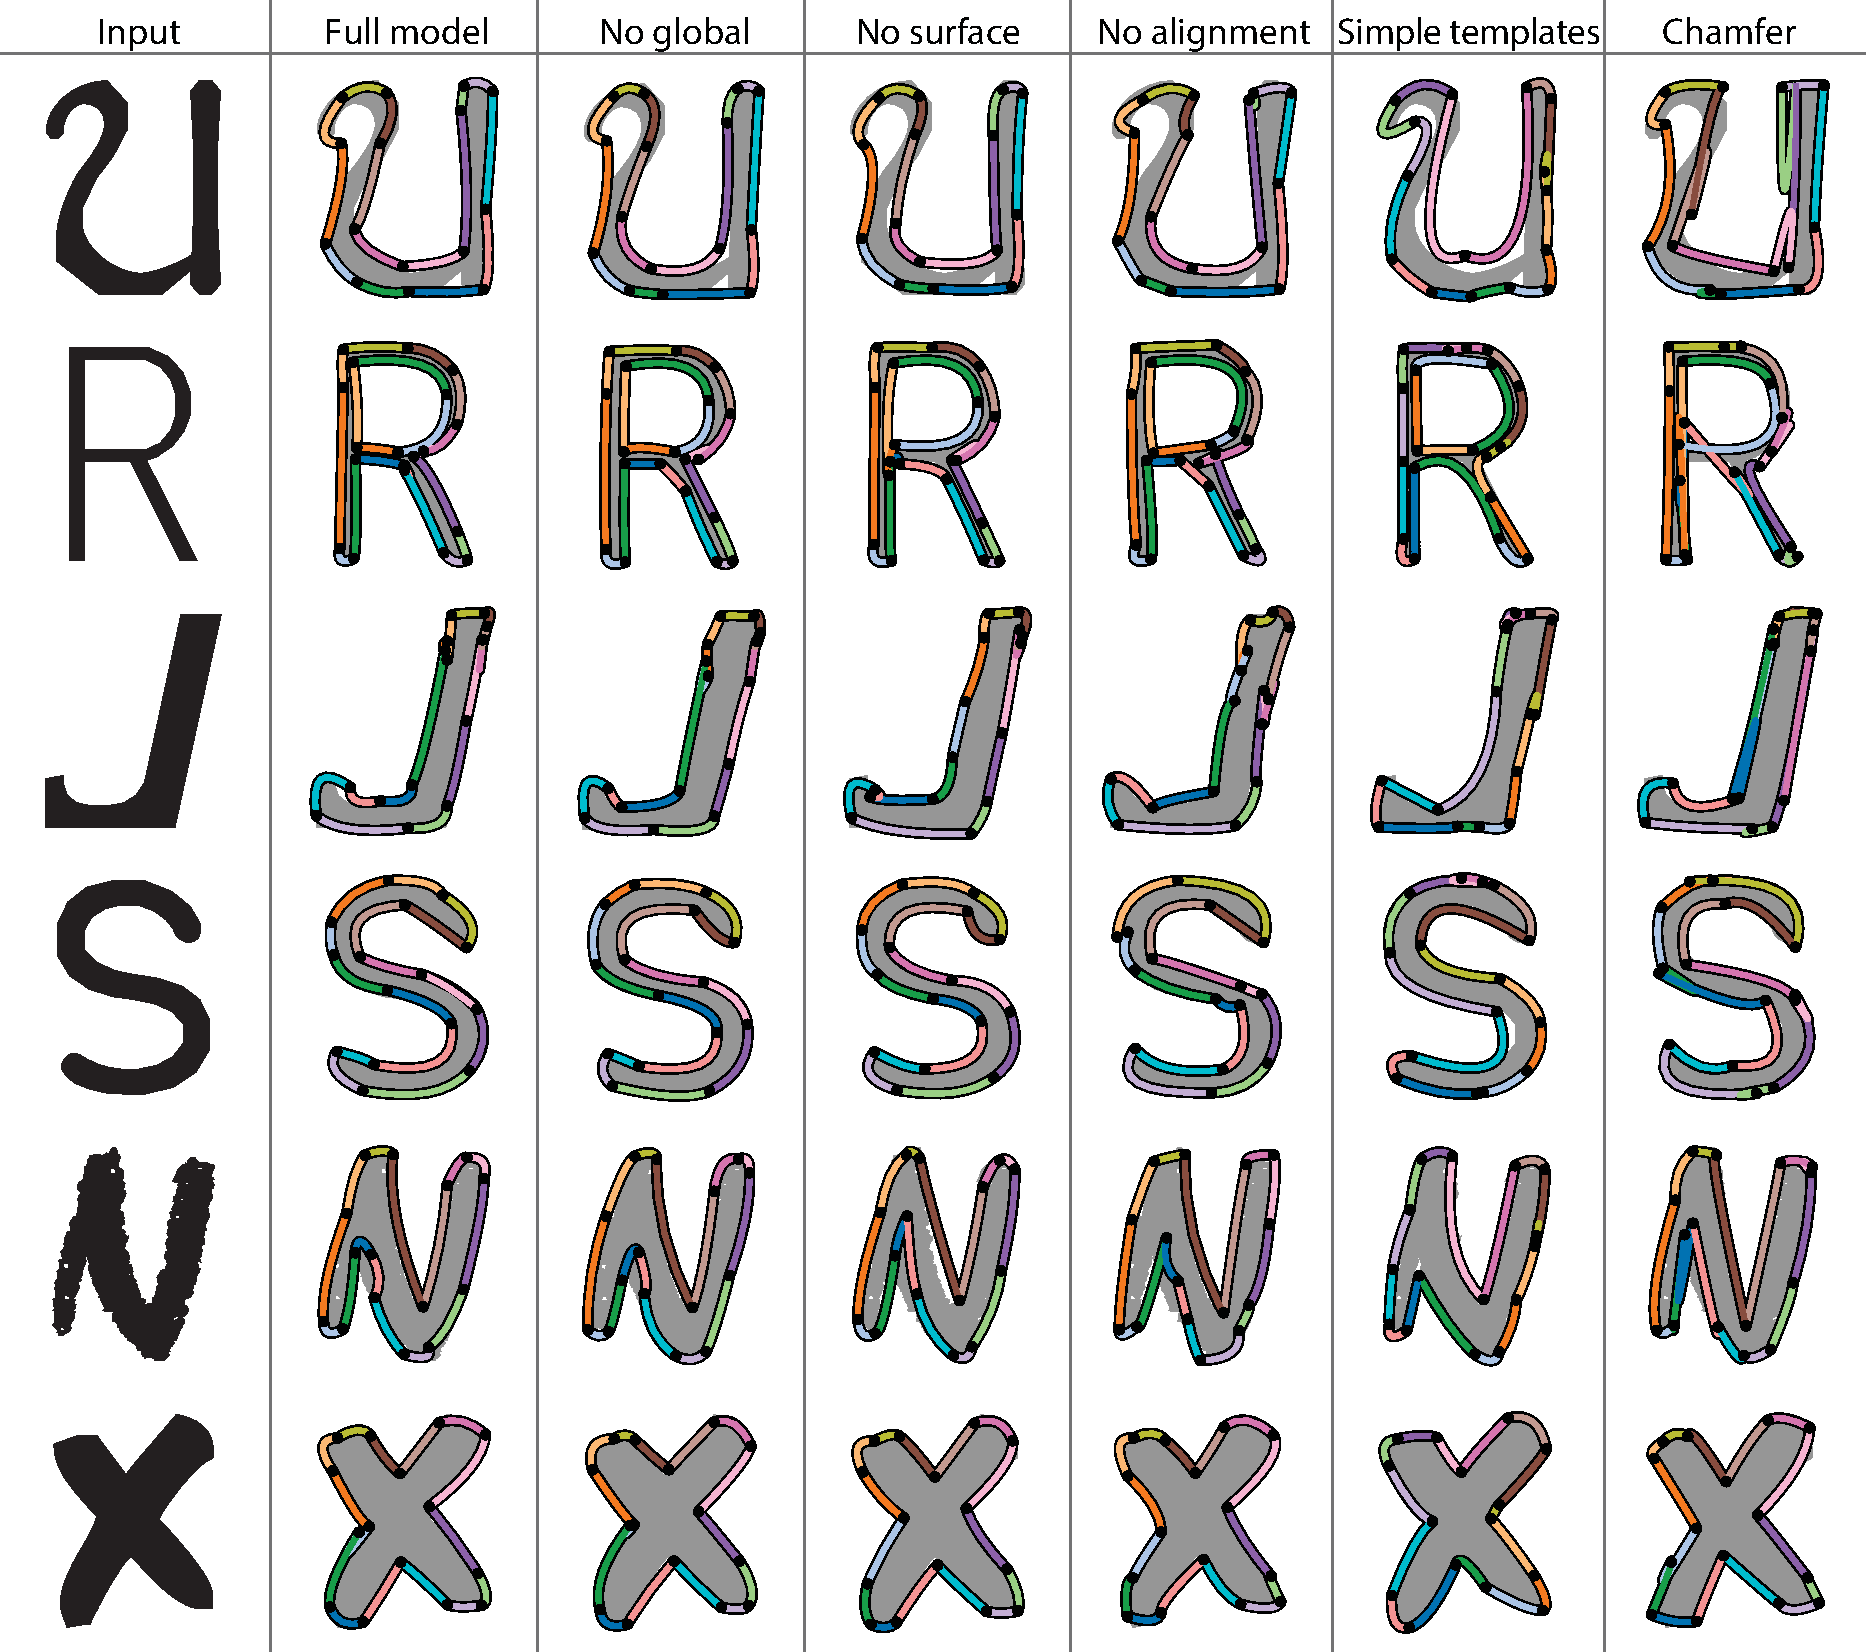
\includegraphics[width=\linewidth]{figures/sup_ablation}
    \caption{Distance field loss comparisons.}
    \label{fig:sup-ablation}
\end{figure*}

\begin{figure*}[t]
    \centering
    \includegraphics[width=.4\linewidth]{figures/loss_convergence}\vspace{-.1in}
    \caption{Local loss (smoothed) over the first 4,000 iterations of training with and without global loss in the objective function. The global loss term results in faster convergence.\vspace{-0.1in}}
    \label{fig:loss_convergence}
\end{figure*}


\begin{figure*}[t!]
    \centering
    \includegraphics[width=\linewidth]{figures/sup_chairs}
    \label{fig:sup-chairs}
    \caption{Cuboid reconstructions of ShapeNet chairs.}
\end{figure*}

\begin{figure*}[t!]
    \centering
    \includegraphics[width=\linewidth]{figures/sup_airplanes}
    \label{fig:sup-airplanes}
    \caption{Cuboid reconstructions of ShapeNet airplanes.}
\end{figure*}

\begin{figure*}[t!]
    \centering
    \includegraphics[width=0.8\linewidth]{figures/sup_seg}
    \label{fig:sup-seg}
    \caption{Cuboid segmentation of Shape COSEG chairs.}
\end{figure*}
\end{document}
